\section{State machines}

A finite state machine is used to visualise a system.
It consists of circles, representing states, and arrows, representing transitions.
Transitions are labelled with the input condition that triggers them.

An abstract machine which can be in only one state at each time.

There are two representations of state machines, Mealy and Moore.

Moore machines have outputs that depend only on the current state.

Mealy machines have outputs that depend on the current state and the current input.


\begin{center}
	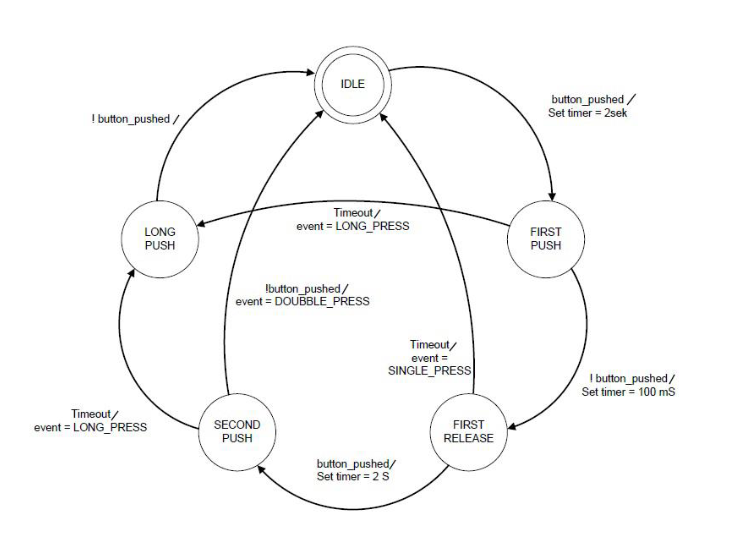
\includegraphics[width=\textwidth]{images/statemachine.png}
\end{center}
